\documentclass[a4paper, 14pt]{extarticle}
\usepackage[settings]{markdown}
\usepackage{minted}

% Поля
%--------------------------------------
\usepackage{geometry}
\geometry{a4paper,tmargin=2cm,bmargin=2cm,lmargin=3cm,rmargin=1cm}
%--------------------------------------


%Russian-specific packages
%--------------------------------------
\usepackage[T2A]{fontenc}
\usepackage[utf8]{inputenc} 
\usepackage[english, main=russian]{babel}
%--------------------------------------

\usepackage{textcomp}

% Красная строка
%--------------------------------------
\usepackage{indentfirst}               
%--------------------------------------             


%Graphics
%--------------------------------------
\usepackage{graphicx}
\graphicspath{ {./images/} }
\usepackage{wrapfig}
%--------------------------------------

% Полуторный интервал
%--------------------------------------
\linespread{1.3}                    
%--------------------------------------

%Выравнивание и переносы
%--------------------------------------
% Избавляемся от переполнений
\sloppy
% Запрещаем разрыв страницы после первой строки абзаца
\clubpenalty=10000
% Запрещаем разрыв страницы после последней строки абзаца
\widowpenalty=10000
%--------------------------------------

%Списки
\usepackage{enumitem}

%Подписи
\usepackage{caption} 

%Гиперссылки
\usepackage{hyperref}

\hypersetup {
	unicode=true
}

%Рисунки
%--------------------------------------
\DeclareCaptionLabelSeparator*{emdash}{~--- }
\captionsetup[figure]{labelsep=emdash,font=onehalfspacing,position=bottom}
%--------------------------------------

\usepackage{tempora}
\usepackage{amsmath}
\usepackage{color}
\usepackage{listings}
\lstset{
  belowcaptionskip=1\baselineskip,
  breaklines=true,
  frame=L,
  xleftmargin=\parindent,
  language=Python,
  showstringspaces=false,
  basicstyle=\footnotesize\ttfamily,
  keywordstyle=\bfseries\color{blue},
  commentstyle=\itshape\color{purple},
  identifierstyle=\color{black},
  stringstyle=\color{red},
}

%--------------------------------------
%			НАЧАЛО ДОКУМЕНТА
%--------------------------------------

\begin{document}

%--------------------------------------
%			ТИТУЛЬНЫЙ ЛИСТ
%--------------------------------------
\begin{titlepage}
\thispagestyle{empty}
\newpage


%Шапка титульного листа
%--------------------------------------
\vspace*{-60pt}
\hspace{-65pt}
\begin{minipage}{0.3\textwidth}
\hspace*{-20pt}\centering

\includegraphics[width=\textwidth]{emblem}
\end{minipage}
\begin{minipage}{0.67\textwidth}\small \textbf{
\vspace*{-0.7ex}
\hspace*{-6pt}\centerline{Министерство науки и высшего образования Российской Федерации}
\vspace*{-0.7ex}
\centerline{Федеральное государственное бюджетное образовательное учреждение }
\vspace*{-0.7ex}
\centerline{высшего образования}
\vspace*{-0.7ex}
\centerline{<<Московский государственный технический университет}
\vspace*{-0.7ex}
\centerline{имени Н.Э. Баумана}
\vspace*{-0.7ex}
\centerline{(национальный исследовательский университет)>>}
\vspace*{-0.7ex}
\centerline{(МГТУ им. Н.Э. Баумана)}}
\end{minipage}
%--------------------------------------

%Полосы
%--------------------------------------
\vspace{-25pt}
\hspace{-35pt}\rule{\textwidth}{2.3pt}

\vspace*{-20.3pt}
\hspace{-35pt}\rule{\textwidth}{0.4pt}
%--------------------------------------

\vspace{1.5ex}
\hspace{-35pt} \noindent \small ФАКУЛЬТЕТ\hspace{50pt} <<Информатика и системы управления>>

\vspace*{-16pt}
\hspace{47pt}\rule{0.83\textwidth}{0.4pt}

\vspace{0.5ex}
\hspace{-35pt} \noindent \small КАФЕДРА\hspace{50pt} <<Теоретическая информатика и компьютерные технологии>>

\vspace*{-16pt}
\hspace{30pt}\rule{0.866\textwidth}{0.4pt}
  
\vspace{11em}

\begin{center}
\Large {\bf Лабораторная работа № 8} \\ 
\large {\bf по курсу <<Алгоритмы компьютерной графики>>}\\
% \large <<Модельно-видовые и проективные пеобразования>>
\end{center}\normalsize

\vspace{8em}


\begin{flushright}
  {Студент группы ИУ9-41Б Горбунов А. Д.\hspace*{15pt} \\
  \vspace{2ex}
  Преподаватель Цалкович П. А.\hspace*{15pt}}
\end{flushright}

\bigskip

\vfill
 

\begin{center}
\textsl{Москва 2024}
\end{center}
\end{titlepage}
%--------------------------------------
%		КОНЕЦ ТИТУЛЬНОГО ЛИСТА
%--------------------------------------

\renewcommand{\ttdefault}{pcr}

\setlength{\tabcolsep}{3pt}
\newpage
\setcounter{page}{2}

\section{Задача}\label{Sect::task}
\par
Переписать на шейдерах одну из лабораторных: 2, 3 или 6.

\section{Теория}\label{Sect::task}
\par

\begin{center}
\Large {Шейдеры} \\ 
\end{center}\normalsize

• шейдер – программа, написанная на языке OpenGL Shader Language и выполняющаяся на GPU

– вершинные шейдеры (vertex shader) – определение положения, цвета, текстурных координат;

– геометрические шейдеры (geometry shader) – обработка примитивов;

– фрагментные/пиксельные шейдеры (fragment/pixel shader) – управление растеризацией;

– тесселяционные шейдеры (OpenGL 4+): (tessellation control shaders = hull shaders, tessellation evaluation shaders = domain shaders) – разбиение граней.

\pagebreak
\section{Код решения}
\begin{minted}{c++}
    Файл main.cpp
#include <GL/glew.h>
#include <GLFW/glfw3.h>
#include <cmath>
#define STB_IMAGE_IMPLEMENTATION
#include "stb_image.h"
#include "iostream"
#include <fstream>
#include <sstream>
using std::cos, std::sin, std::string;
using namespace std::string_literals;
int mode = 1;
int lightMode = 1;
int degreeMode = 1;
int timeMode = 0;
float degree_y = 0.0;   
float degree_x = 0.0;
float move_y = 0.0;
float move_x = 0.0;
float osnov_x = 0.1;
float osnov_y = 0.0;
float flying_speed = 0;
float V = 3.14 * pow(10,-4);
float acl = pow(10,-4);
int width = 1000;
int height = 1000;
GLuint textureID;
void key_callback(GLFWwindow *window, int key, int scancode, int action, int mods)
{
    if (action == GLFW_PRESS || action == GLFW_REPEAT)
    {
        if (key == GLFW_KEY_ESCAPE)
        {
            glfwSetWindowShouldClose(window, GL_TRUE);
        }
        else if (key == GLFW_KEY_UP)
        {
            degree_y += 0.2;
        }
        else if (key == GLFW_KEY_DOWN)
        {
            degree_y -= 0.2;
        }
        else if (key == GLFW_KEY_LEFT)
        {
            degree_x += 0.2;
        }
        else if (key == GLFW_KEY_RIGHT)
        {
            degree_x -= 0.2;
        }
        else if (key == GLFW_KEY_D)
        {
            move_x += 0.2;
        }
        else if (key == GLFW_KEY_A)
        {
            move_x -= 0.2;
        }
        else if (key == GLFW_KEY_W)
        {
            move_y += 0.2;
        }
        else if (key == GLFW_KEY_S)
        {
            move_y -= 0.2;
        }
        else if (key == GLFW_KEY_L)
        {
            osnov_x += 0.1;
        }
        else if (key == GLFW_KEY_K)
        {
            osnov_x -= 0.1;
        }
        else if (key == GLFW_KEY_I)
        {
            osnov_y += 0.1;
        }
        else if (key == GLFW_KEY_O)
        {
            osnov_y -= 0.1;
        }
        else if (key == GLFW_KEY_SPACE) 
        {
            mode = (mode + 1) % 2;
            if (mode == 0)
                glPolygonMode(GL_FRONT_AND_BACK, GL_LINE);
            else 
                glPolygonMode(GL_FRONT_AND_BACK, GL_FILL);  
        }
        else if (key == GLFW_KEY_1)
        {
            lightMode = (lightMode + 1) % 2;
            glDisable(GL_LIGHT0);
        }
        else if (key == GLFW_KEY_2)
        {
            degreeMode = (degreeMode + 1) % 2;
        }
        else if (key == GLFW_KEY_3)
        {
            timeMode = (timeMode + 1) % 2;
        }
    }
}
void light()
{
    glPushMatrix();
    glLoadIdentity();
    glTranslatef(1, 1, 1);
    GLfloat material_diffuse[] = {0.75, 0.75, 0.75, 0.0};
    glMaterialfv(GL_FRONT_AND_BACK, GL_DIFFUSE, material_diffuse);
    GLfloat light2_diffuse[] = {1, 1, 0};
    GLfloat light2_position[] = {0, 0, 0, 1.0};
    glEnable(GL_LIGHT0);
    glLightfv(GL_LIGHT0, GL_DIFFUSE, light2_diffuse);
    glLightfv(GL_LIGHT0, GL_POSITION, light2_position);
    glLightf(GL_LIGHT0, GL_CONSTANT_ATTENUATION, 0.0);
    glLightf(GL_LIGHT0, GL_LINEAR_ATTENUATION, 0.2);
    glLightf(GL_LIGHT0, GL_QUADRATIC_ATTENUATION, 0.4);
    glPopMatrix();
}
void texture()
{
    int width_1, height_1, channels;
    unsigned char* image = stbi_load("./../texture.bmp", &width_1, &height_1, &channels, 0);
    glEnable(GL_TEXTURE_2D);
    glGenTextures(1, &textureID);
    glBindTexture(GL_TEXTURE_2D, textureID);
    glTexParameterf(GL_TEXTURE_2D, GL_TEXTURE_WRAP_S, GL_REPEAT);
    glTexParameterf(GL_TEXTURE_2D, GL_TEXTURE_WRAP_T, GL_REPEAT);
    glTexParameterf(GL_TEXTURE_2D, GL_TEXTURE_MAG_FILTER, GL_NEAREST);
    glTexParameterf(GL_TEXTURE_2D, GL_TEXTURE_MIN_FILTER, GL_NEAREST);
    if (image){
        glTexImage2D(GL_TEXTURE_2D, 0, GL_RGB, width_1, height_1, 0, GL_RGB, GL_UNSIGNED_BYTE, image);
    }
   stbi_image_free(image);
}
void move_object()
{
    flying_speed -= V;
    V += acl;
    if(flying_speed < -2.2 or flying_speed > 2.2)
        V = -V;
}
void display(GLFWwindow* window)
{
    glClearColor (0.3, 0.3, 0.3, 0.0);
    glEnable(GL_DEPTH_TEST);
    glClear(GL_COLOR_BUFFER_BIT | GL_DEPTH_BUFFER_BIT);
    glBindTexture(GL_TEXTURE_2D, textureID);
    glPushMatrix();
    glTranslatef(0.0f + move_x, 0.0f + move_y + flying_speed, 0.0f);
    glRotatef(degree_y * 50.f, 1.f, 0.f, 0.f);
    glRotatef(degree_x * 50.f, 0.f, 1.f, 0.f);
    glBegin(GL_QUAD_STRIP);
    glColor3f(0.4f, 0.4f, 1.0f);
    for (int i = 0; i <= 360; i += 10)
    {
        float angle = i * M_PI / 180 ;
        glTexCoord2f(1 * cos(angle) + osnov_x, 0.5 * sin(angle) + osnov_y);
        glVertex3f(1 * cos(angle) + osnov_x, 0.5 * sin(angle) + osnov_y, 0.0);
        glTexCoord2f(1 * cos(angle), 0.5 * sin(angle));
        glVertex3f(1 * cos(angle), 0.5 * sin(angle), 1);
    }
    glEnd();
    glBegin(GL_POLYGON);
    glNormal3f(1, 1, -1);
    glColor3f(1.0f, 0.3f, 0.3f);
    for (int i = 0; i <= 360; i++)
    {
        float angle = i * M_PI / 180;
        glTexCoord2f(1 * cos(angle) + osnov_x, 0.5 * sin(angle) + osnov_y);
        glVertex3f(1 * cos(angle) + osnov_x, 0.5 * sin(angle) + osnov_y, 0.0);
    }
    glEnd();
    glBegin(GL_POLYGON);
    glNormal3f(1, 1, 1);
    glColor3f(0.5f, 0.7f, 0.7f);
    for (int i = 0; i <= 360; i++)
    {
        float angle = i * M_PI / 180;
        glTexCoord2f(1 * cos(angle), 0.5 * sin(angle));
        glVertex3f(1 * cos(angle), 0.5 * sin(angle), 1);
    }
    glEnd();
    glPopMatrix();
    GLfloat spec[] = {1, 1, 1, 1};
    GLfloat emiss[] = {0, 0, 0, 1};
    GLfloat shin = 50;
    glColorMaterial(GL_FRONT_AND_BACK, GL_AMBIENT_AND_DIFFUSE);
    glMaterialfv(GL_FRONT_AND_BACK, GL_SPECULAR,  spec);
    glMaterialfv(GL_FRONT_AND_BACK, GL_SHININESS, &shin);
    glMaterialfv(GL_FRONT_AND_BACK, GL_EMISSION,  emiss);
}
GLuint compileShader(GLuint type, const std::string& source)
{
    GLuint id = glCreateShader(type);
    const char* src = source.c_str();
    glShaderSource(id, 1, &src, nullptr);
    glCompileShader(id);

    int result;
    glGetShaderiv(id, GL_COMPILE_STATUS, &result);
    if (result == GL_FALSE)
    {
        int length;
        glGetShaderiv(id, GL_INFO_LOG_LENGTH, &length);
        char* message = (char*)alloca(length * sizeof(char));
        glGetShaderInfoLog(id, length, &length, message);
        std::cout << "Failed to compile " << (type == GL_VERTEX_SHADER ? "vertex" : "fragment") << " shader!" << std::endl;
        std::cout << message << std::endl;
        glDeleteShader(id);
        return 0;
    }
    return id;
}
int main()
{
    if (!glfwInit()) {
        return -1;
    }
    GLFWwindow* window = glfwCreateWindow(width, height, "Lab 8", NULL, NULL);
    if (!window) {
        glfwTerminate();
        return -1;
    }
    glViewport(0, 0, width, height);

    glfwMakeContextCurrent(window);
    glfwSetKeyCallback(window, key_callback);

    GLenum err = glewInit();
    if (err != GLEW_OK) {
        std::cerr << "Failed to initialize GLEW: " << glewGetErrorString(err) << std::endl;
        return -1;
    }
    string vertexShaderSource =
"attribute vec3 aVert; "s+
"varying vec3 n; "s+
"varying vec3 v; "s+
"varying vec2 uv;"s+
"varying vec4 vertexColor; "s+
"void main() {"s+
"    uv = gl_MultiTexCoord0.xy; "s+
"    v = vec3(gl_ModelViewMatrix * gl_Vertex); "s+
"    n = normalize(gl_NormalMatrix * gl_Normal); "s+
"    gl_TexCoord[0] = gl_TextureMatrix[0]  * gl_MultiTexCoord0; "s+
"    gl_Position = gl_ModelViewProjectionMatrix * vec4(gl_Vertex.x, gl_Vertex.y, gl_Vertex.z, 1); "s+
"    vec4 vertexColor = vec4(0.5f, 0.0f, 0.0f, 1.0f);"s+
"}"s;
    string fragmentShaderSource =
"varying vec3 n; "s+
"varying vec3 v; "s+
"varying vec4 vertexColor;"s+
"uniform sampler2D tex; "s+
"void main () {  "s+
"    vec3 L = normalize(gl_LightSource[0].position.xyz - v); "s+
"    vec3 E = normalize(-v); "s+
"    vec3 R = normalize(-reflect(L,n)); "s+
"    vec4 Iamb = gl_FrontLightProduct[0].ambient; "s+
"    vec4 Idiff = gl_FrontLightProduct[0].diffuse * max(dot(n,L), 1.0); "s+
"    Idiff = clamp(Idiff, 2.0, 0.6);     "s+
"    vec4 Ispec = gl_LightSource[0].specular * pow(max(dot(R,E),0.0),0.7);"s+
"    Ispec = clamp(Ispec, 0.0, 1.0); "s+
"    vec4 texColor = texture2D(tex, gl_TexCoord[0].st); "s+
"    gl_FragColor = (Idiff + Iamb + Ispec) * texColor;"s+
"}"s;
    string fragmentShaderSource_bad =
"varying vec3 n; "s+
"varying vec3 v; "s+
"varying vec4 vertexColor;"s+
"uniform sampler2D tex; "s+
"void main () {  "s+
"    vec3 L = normalize(gl_LightSource[0].position.xyz - v); "s+
"    vec3 E = normalize(-v); "s+
"    vec3 R = normalize(-reflect(L,n)); "s+
"    vec4 Iamb = gl_FrontLightProduct[0].ambient; "s+
"    vec4 Idiff = gl_FrontLightProduct[0].diffuse * max(dot(n,L), 0.0); "s+
"    Idiff = clamp(Idiff, 0.0, 1.0);     "s+
"    vec4 Ispec = gl_LightSource[0].specular * pow(max(dot(R, E), 0.0), gl_FrontMaterial.shininess);"s+
"    Ispec = clamp(Ispec, 0.0, 1.0); "s+
"    vec4 texColor = texture2D(tex, gl_TexCoord[0].st); "s+
"    gl_FragColor = (Idiff + Iamb + Ispec) * texColor;"s+
"}"s;
    GLuint vertex = compileShader(GL_VERTEX_SHADER, vertexShaderSource);
    GLuint fragment = compileShader(GL_FRAGMENT_SHADER, fragmentShaderSource);
    //GLuint fragment = compileShader(GL_FRAGMENT_SHADER, fragmentShaderSource_bad); 
    int program = glCreateProgram();
    glAttachShader(program, vertex);
    glAttachShader(program, fragment);
    glLinkProgram(program);
    glScalef(0.25,0.25, 0.25);
    glEnable(GL_LIGHTING);
    glLightModelf(GL_LIGHT_MODEL_TWO_SIDE, GL_TRUE);
    glEnable(GL_NORMALIZE);
    glPolygonMode(GL_FRONT_AND_BACK, GL_FILL);
    texture();
    glUseProgram(program);
    while (!glfwWindowShouldClose(window))
    {
        display(window);
        if(degreeMode)
        {
            degree_x += 0.01;
        }
        if(timeMode)
        {
            move_object();
        }
        if(lightMode)
        {
            light();
        }
        glfwSwapBuffers(window);
        glfwPollEvents();
    }
    glfwTerminate();
    return 0;
}
\end{minted}

\section{Заключение}

    В данной работе я изучил возможности языка C++ в работе с библиотекой OpenGL, а именно научился применять шейднры с помощь функций: glewInit(), lCreateShader(type), glShaderSource(id, 1, src, nullptr), glCompileShader(id), glGetShaderiv(id, GL COMPILE STATUS, result), glCreateProgram(), glAttachShader(program, vertex), glLinkProgram(program), glUseProgram(program).

\section{Результат запуска}
    
\begin{figure}[!htb]
	\centering
	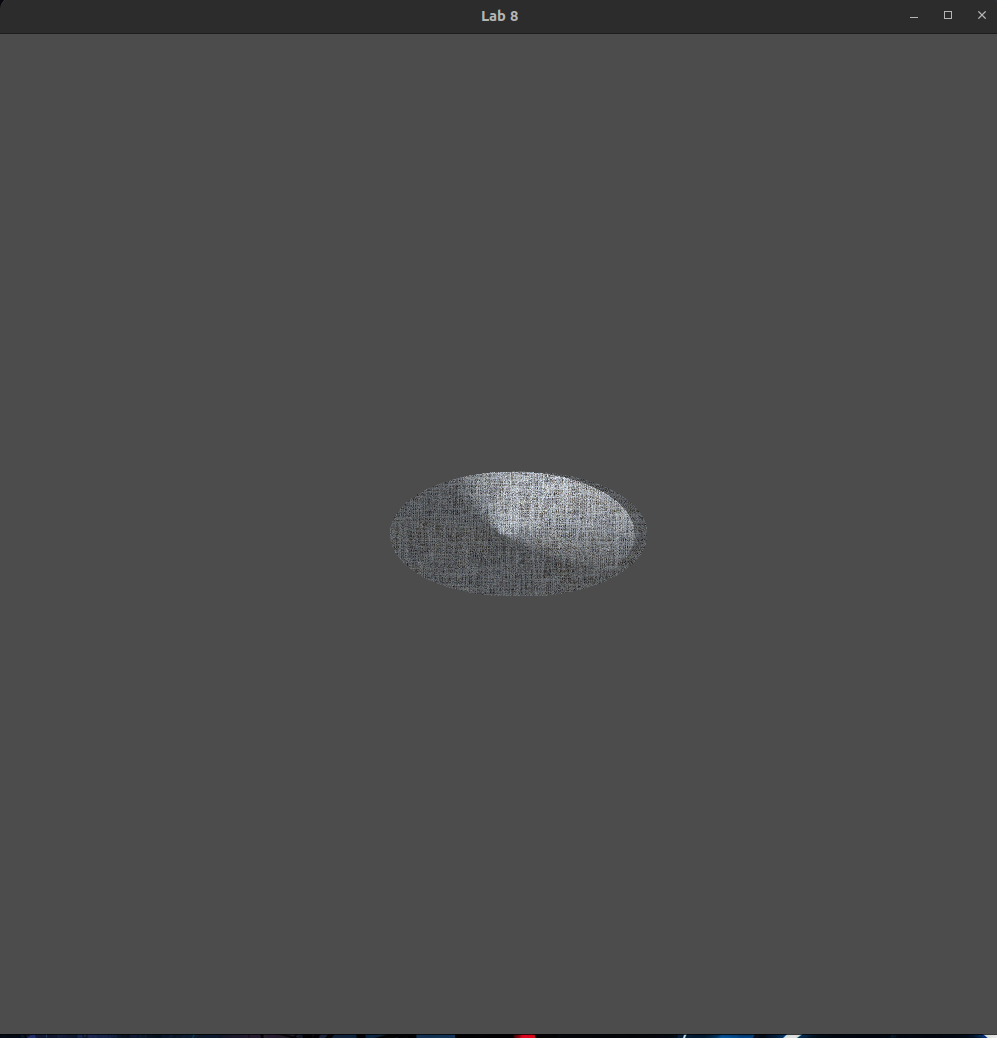
\includegraphics[width=0.8\textwidth]{picture_1.png}
\caption{Шейдер с текстурой 1}
\label{fig:picture_1.png}
\end{figure}

\begin{figure}[!htb]
	\centering
	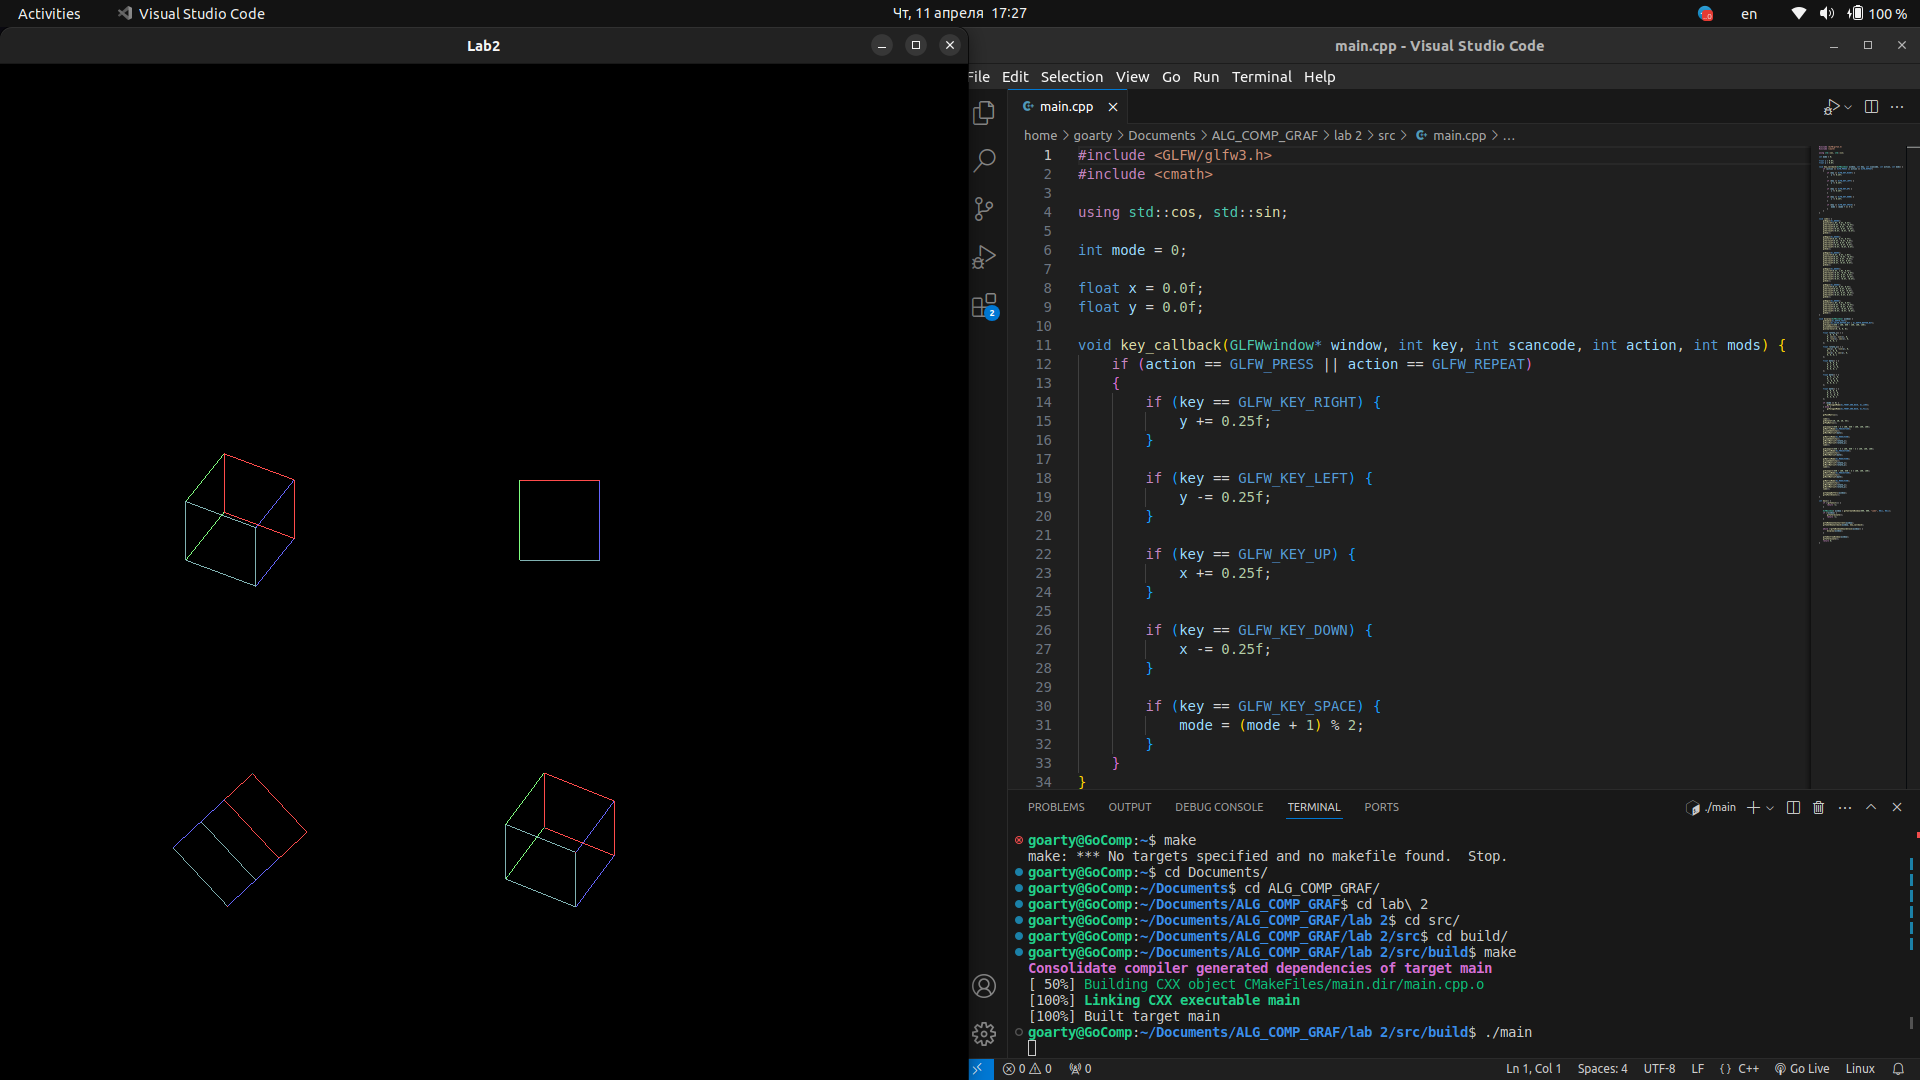
\includegraphics[width=0.8\textwidth]{picture_2.png}
\caption{Шейдер с текстурой 2}
\label{fig:picture_2.png}
\end{figure}

\end{document}

